% Filename  : samplepaper.tex
% Purpose   : A sample exam paper to demonstrate how to use the 'ditpaper'
%             TeX class.
% Author    : Emmet Caulfield
% Revision  : $Id: samplepaper.tex 2 2006-02-19 20:34:45Z emmet $
% Repository: $HeadURL: http://svn.netrogen.lan/tex-ditpaper/trunk/samplepaper.tex $
%

% 'nosolution' (default) and 'solution' toggle the inclusion of solutions
% in the output. The tag --SOLUTION-OPTION--, below, is replaced by 'sed' 
% in the Makefile to cause both the paper and the solutions to be produced.
\documentclass[--SOLUTION-OPTION--]{ditpaper}

\usepackage{graphicx}
\usepackage{multirow}
\usepackage{rotating}


% These must be set or bizarre defaults will be used:
\facility{Kevin Street, Dublin 8}
\course{BSc (Hons) in Computer Science}
\examcode{R228/406}
\stage{Stage 4}
\session{Supplemental Examinations 2011}
\title{Artificial Intelligence II}
\examiners{Dr. John Kelleher\\
Dr. D. Lillis\\
Dr. I. Arana}
\examdate{}
\examtime{Duration: 2 Hours}
\instructions{Answer Question 1 (40 marks) \textbf{and}\par{} any 2 Other Questions (30 marks each).}


\begin{document}


%aima chapters 18
% inductive bias, learning theory - supervised/unsupervised, overfitting, lazy/eager learner, classification v regression, false positive v false negatives, linear separability, consistency, evaluation

\question
\begin{enumerate}
	\item Explain what is meant by \textbf{inductive learning}.
	\marks{5}
	\begin{answer}
		Inductive Learning involves the process of learning by example � where a system tries to induce a general rule from a set of observed instances
	\end{answer}
	\item In the context of machine learning, explain what is meant by \textbf{overfitting} the training data.
	\marks{5}
	\begin{answer}
		Overfitting occurs when classifiers make decisions based on accidental properties of the training set that will lead to errors on the test set (or new data). As a result, whenever there is a large set of possible hypotheses, one has to be careful not to use the resulting freedom to find meaningless "regularity" in the data.
	\end{answer}
	\item  In the context of machine learning, explain what is meant by the term \textbf{inductive bias} and illustrate your explaination using examples of inductive biases used by machine learning algorithms.
	\marks{10}
	\begin{answer}
		\begin{itemize}
				\item The inductive bias of a learning algorithm:
				\begin{enumerate}
					\item is a set of assumption about what the true function we are trying to model looks like.
					\item defines the set of hypotheses that a learning algorithm considers when it is learning.
					\item guides the learning algorithm to prefer one hypothesis (i.e. the hypothesis that best fits with the assumptions) over the others. 
					\item is a necessary prerequisite for learning to happen because inductive learning is an ill posed problem. 
				\end{enumerate}	
				\item An example of the specific inductive bias introduced by particular machine learning algorithms would be good here. E.g.:			
				\begin{itemize}
					\item Maximum margin: when drawing a boundary between two classes, attempt to maximize the width of the boundary. This is the bias used in Support Vector Machines. The assumption is that distinct classes tend to be separated by wide boundaries.
					\item Minimum cross-validation error: when trying to choose among hypotheses, select the hypothesis with the lowest cross-validation error.
				\end{itemize}
			\end{itemize}
	\end{answer}
	\item Let us say we have three classification algorithms. How can we order these three from best to worst?
	\marks{20}
	\begin{answer}
		This is a discursive question so giving a precise answer is not appropriate. However, key points that the student should touch on include:
		\begin{itemize}
		\item Predictive accuracy
		\item Speed and scalability 
		\begin{itemize}
			\item Time to construct the model
			\item Time to use the model
		\end{itemize}
		\item Robustness (handling noise and missing values)
		\item Scalability
		\item Interpretability (understanding and insight provided by the model)
	\end{itemize}
	It should be noted also, that these evaluation criteria are application dependent.
	\end{answer}
\end{enumerate}


\newpage

%Q2
% knn and CBR 
% information theory, entropy, Decision Trees, Inductive logic programming
\begin{table}[htdp]
\caption{Example feature vectors for animal classification. A 1 indicates the animal possesses the feature listed in the column, and 0 indicates they do not. The rightmost column lists the classification of each ainmal.}
\begin{center}
\begin{tabular}{|c|c|c|c|c|c|c|c|c|c|c|}
\hline
Species & \begin{sideways}Births Live Young\end{sideways} & \begin{sideways}Lays Eggs\end{sideways} & \begin{sideways}Feeds Offspring Own Milk\end{sideways} & \begin{sideways}Warm-Blooded\end{sideways}  & \begin{sideways}Cold-Blooded \end{sideways} & \begin{sideways}Land and Water Based\end{sideways} & \begin{sideways}Has Hair \end{sideways} & \begin{sideways}Has Feathers\end{sideways} & Class \\
\hline 
Cat & 1 & 0 & 1 & 1 & 0 & 0 & 1 & 0 & Mammal \\
Frog & 0 & 1 & 0 & 0 & 1 & 1 & 0 & 0 & Amphibian \\
Squirrel & 1 & 0 & 1 & 1 & 0 & 0 & 1 & 0 & Mammal \\
Duck & 0 & 1 & 0 & 1 & 0 & 1 & 0 & 1 & Bird \\
\hline
\end{tabular}
\end{center}
\label{tab:ainmals-classification}
\end{table}%

\begin{table}[htdp]
\caption{The attributes of a newly discovered animal. A 1 indicates the animal possesses the feature listed in the column, and 0 indicates they do not. The column on the right contains a ? because the animal has not yet been classified.}
\begin{center}
\begin{tabular}{|c|c|c|c|c|c|c|c|c|c|c|}
\hline
Species & \begin{sideways}Births Live Young\end{sideways} & \begin{sideways}Lays Eggs\end{sideways} & \begin{sideways}Feeds Offspring Own Milk\end{sideways} & \begin{sideways}Warm-Blooded\end{sideways}  & \begin{sideways}Cold-Blooded \end{sideways} & \begin{sideways}Land and Water Based\end{sideways} & \begin{sideways}Has Hair \end{sideways} & \begin{sideways}Has Feathers\end{sideways} & Class \\
\hline 
Mystery & 0 & 1 & 0 & 0 & 0 & 1 & 0 & 0 & ? \\
\hline
\end{tabular}
\end{center}
\label{tab:animal-attributes}
\end{table}%
		
			
\question 
	\begin{enumerate}
		\item You are working as an assistant-biologist to the Charles Darwin on the Beagle voyage. You are at the Gal\'apagos Islands and you have just discovered a new animal that has not yet been classified. Table \ref{tab:animal-attributes} lists the attributes of the animal you have found. Mr. Darwin has asked you to classify the animal using a nearest-neighbour approach and he has supplied you with a case-base of already classified animals, see Table \ref{tab:ainmals-classification}. 
		\begin{enumerate}
			\item A good measure of distance between two instances with categorical features is the number of features which have different values (the \textbf{overlap metric}, also known as the \textbf{hamming distance}). Using this measure of distance compute the distances between the mystery animal and each of the animals in the case base. 
		\marks{5}
		\begin{answer}
				\begin{center}
					\begin{tabular}{|c|c|c|}
						\hline
						Species & Class & Distance\\
						\hline 
						Cat & Mammal & 6\\
						Frog & Amphibian & 1\\
						Squirrel & Mammal & 6\\
						Duck & Bird & 2\\
						\hline
					\end{tabular}
				\end{center}
		\end{answer}
			\item If you used \textit{1-NN} classification what class would be assigned to the mystery animal.
		\marks{5}
		\begin{answer}
			The nearest neighbor to the mystery animal is the Frog. So the mystery animal would be classified as an amphibian.
		\end{answer}
			\item If the you used \textit{4-NN} classification what class would be assigned to the mystery animal. 
		\marks{5}
		\begin{answer}
				If you applied a \textit{4-NN} classification to this case-base you would include all the instances in the case-base irrespective of their distance from the test instance feature vector. As a result the test instance would be assigned the most frequently occurring class in the case-base. This would result in the mystery animal being classified as a mammal. 
		\end{answer}
		\end{enumerate}
		% Information theory and Decision Trees
		\item In the context of Decision Tree Learning define what is meant by the following terms:
			\begin{enumerate}
			%Callan
					\item entropy
					\marks{5}					
					\begin{answer}
				For $c$ classification categories the entropy $E$ is defined as: $E=\sum_{i=1}^{c} -p_i\ log_2\ p_i$ where $p_i$ is the probability of category $i$ occurring.
					\end{answer}
			%Callan
			\item information gain
					\marks{5}
			\begin{answer}
				The information gain for an attribute is the expected reduction in entropy if the examples were to be partitioned according to that attribute and is defined as: $Gain(T,A)=E(T) - \sum_{j=1}^{v} \frac{|T_{j}|}{|T|}E(T_{j})$ where $T$ is a set of training examples and $T_j$ is a subset of examples having value $j$ for attribute $A$ 
			\end{answer}
			\end{enumerate}
		%inductive logic programming
		\item The FOIL inductive logic programming algorithm is constructing a new rule with head $p(Y) \leftarrow$. Which of the following literals could be considered as candidate extensions $q(Y)$, $r(X)$, $s(X,Y)$, $\lnot s(X,Y)$?
			\marks{5}
\begin{answer}
Three of the given literals could be considered as extensions: $q(Y)$, $s(X,Y)$, $\lnot s(X,Y)$. The literal $r(X)$ would not be considered as an extension as it does not contain at least one variable that is already present in the rule.
\end{answer}
	\end{enumerate}



\newpage
	
%Q3 30 marks
% basic probability 5
% bayesian networks 10
% bayesian learning  15

\question
	\begin{enumerate}
		%basic probability
		\item Given that $P(a|b)=0.5$, $P(a)=0.3$, $P(b)=0.4$ calculate $P(b|a)$.
			\marks{5}
			\begin{answer}
				$P(b|a)=\frac{P(a|b)\times P(b)}{P(a)}=\frac{0.5 \times 0.4}{0.3}=0.67$
			\end{answer}
		%bayesian networks
		\item In you local power station, there is an alarm that senses when a temperature gauge exceeds a given threshold. The gauge measures the temperature of the core. Consider the Boolean variables $A$ (alarm sounds), $F_A$ (alarm is faulty), and $F_G$ (gauge is faulty); and multivalued nodes $G$ (gauge reading) and $T$ (actual core temperature).
		\begin{enumerate}
			\item Draw a Bayesian network for this domain, given that the gauge is more likely to fail when the core temperature gets too high.
			\marks{5}
			\begin{answer}
				The key aspects are: the failure nodes are parents of the sensor nodes, and the temperature node is a parent of both the gauge and the gauge failure node. It is exactly this kind of correlation that makes it dif�cult for humans to understand what is happening in complex systems with unreliable sensors.
				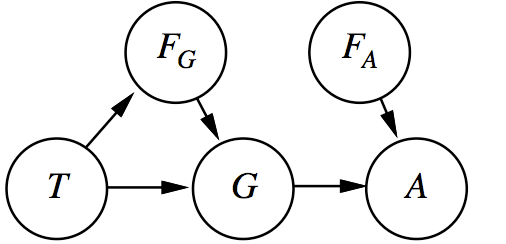
\includegraphics[width=\textwidth]{./images/nuclearpowerstationbayesiannet.png}
			\end{answer}
			\item Suppose there are just two possible actual and measured temperatures, normal and high and the probability that the gauge gives the correct temperature is $x$ when it is working, but $y$ when it is faulty. Give the conditional probability table associated with node $G$.
			\marks{5}
			\begin{answer}
				Note the semantics of $F_G$ , which is true when the gauge is faulty, i.e., not working.
				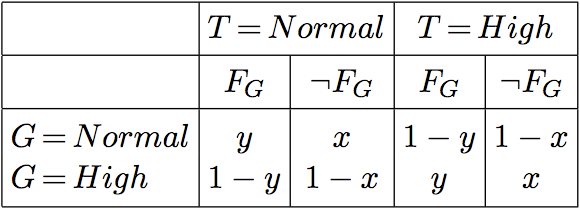
\includegraphics[width=\textwidth]{./images/cpt_node_g_q142.png}
			\end{answer}
		\end{enumerate}
		%bayesian learning
		\item You are on holidays on Fisher Island. The yearly weather on Fisher Island comes in five different varieties: 
			\begin{itemize}
				\item there is a 10\% chance that there will be rain everyday of the year.
				\item there is a 20\% chance that there will be rain on 75\% of the days of the year.
				\item there is a 40\% chance that there will be rain on 50\% of the days of the year.
		    		 \item there is a 20\% chance that there will be rain on 25\% of the days of the year.
		     		\item there is a 10\% chance that there will be no rain on any day of the year.
			\end{itemize}
			\begin{enumerate}
				\item Given that it has rained on day 1 and 2 of the year compute the posterior probability of each of the 5 yearly weather patterns on day 2 of the year. Give your answer rounded to four places of precision.
				\marks{10}
				\begin{answer}
						To begin we will define some notation. Let: 
						\begin{itemize}
							   \item $h_1$ denote the hypothesis that it will rain everyday, $P(h_1)=0.1$.
					\item $h_2$ denote the hypothesis that it will rain on 75\% of the days of the year, with prior $P(h_2)=0.2$.
					\item $h_3$ denote the hypothesis that it will rain on 50\% of the days of the year, with prior $P(h_3)=0.4$.
					\item $h_4$ denote the hypothesis that it will rain on 25\% of the days of the year, with prior $P(h_4)=0.2$.
					\item $h_5$ denote the hypothesis that there will be no rain during the year, with prior $P(h_5)=0.1$.
					\end{itemize}
					Also, if we use the notation $rain_x$ to represent the observation of rain on day x of the year, then the probability of rain on a day of the year given a particular hypothesis $h$ is:
					\begin{itemize}
						\item $P(rain_x|h_1)=1.0$ .
						\item $P(rain_x|h_2)=0.75$ .
						\item $P(rain_x|h_3)=0.5$ .
						\item $P(rain_x|h_4)=0.25$ .
						\item $P(rain_x|h_5)=0.0$ .
					\end{itemize}
					Then:
						\begin{itemize}
							\item By Bayes' rule, we can compute the posterior probability of a hypothesis given the data so far using: $P(h_i|\textbf{d}) = \alpha P(\textbf{d}|h_i) P(h_i)$
				      		\item And, the likelihood of the data given a hypothesis is calculated using: $P(\textbf{d}|h_i) = \prod_j P(d_j|h_i)$
				           \end{itemize}
				       So:
				\begin{itemize}
					\item $P(h_1|rain_1,rain_2)=\alpha (\prod_{j=1}^2 P(rain_j|h_1))P(h_1)=\alpha 1.00^2 \times 0.1=\alpha 0.1=\frac{0.1}{0.325} \approx .3077$.
					\item $P(h_2|rain_1,rain_2)=\alpha (\prod_{j=1}^2 P(rain_j|h_2))P(h_1)=\alpha 0.75^2 \times 0.2=\alpha 0.1125=\frac{0.1125}{0.325} \approx .3461$.
					\item $P(h_3|rain_1,rain_2)=\alpha (\prod_{j=1}^2 P(rain_j|h_3))P(h_1)=\alpha 0.50^2 \times 0.4=\alpha 0.1=\frac{0.1}{0.325} \approx .3077$.
					\item $P(h_4|rain_1,rain_2)=\alpha (\prod_{j=1}^2 P(rain_j|h_4))P(h_1)=\alpha 0.25^2 \times 0.2=\alpha 0.0125=\frac{0.0125}{0.325} \approx .0385$.
					\item $P(h_5|rain_1,rain_2)=\alpha (\prod_{j=1}^2 P(rain_j|h_5))P(h_1)=\alpha 0.00^2 \times 0.1=\alpha 0.0=0.0$.
				\end{itemize}
			\end{answer}
			\item Given that after the first 10 days of the year the weather has been such that the posterior probabilities of each of the 5 varieties of the yearly weather on Fisher Island are:  
					\begin{itemize}
						\item there is now a 90\% chance that there will be rain everyday for the rest of the year; 
						\item a 7\% chance that there will be rain on 75\% of the rest of the days of the year;  
						\item a 2\% chance that there will be rain on 50\% of the rest of the days of the year; 
						\item a 1\% chance that there will be rain on 25\% of the rest of the days of the year; 
						\item and there is a 0\% chance that there will be no rain for the rest of the year. 
					\end{itemize}
					What is the Maximum a Posterior (MAP) probability of rain on day 11?
							   \marks{5}
				         \begin{answer}
				         A MAP prediction just uses the prediction provided by the single most probable hypothesis. In this instance the single most probable hypothesis is the hypothesis that it will rain on every day of the year. This hypothesis would predict rain on day 11 with probability of 1.0 (i.e. certainty)
				         \end{answer}
		\end{enumerate}
	\end{enumerate} %end Q3

%
\newpage

%Q4
%Linear Regression Neural Nets, SVMs, Ensemble Learning
\question 
	\begin{enumerate}
		%Regression Learning
		\item The following model is commonly used for continuous prediction tasks:
		\begin{center}
			$y(x)=w_0 + w_1x_1 + \dots + w_Dx_D$
		\end{center}
		\begin{enumerate}
			\item Provide the name for this model and explain all terms.
			\marks{5}
			\begin{answer}
			Students should explain that this is a simple linear regression model which can be effectively used to make predictions. $x$ is a vector of feature values for a query instance and $w$ is a vector of feature weights. An diagram of a simple one dimensional linear function would help.
			\end{answer}
			\item Explain how the following model can overcome some of the limitations of the model given above. 
\begin{center}
$y(x)=\sum_{j=0}^{M - 1}w_j{\phi}_j(x)$
\end{center}
					\marks{5}
		\begin{answer}
		Students should explain that the simple linear regression model is attractive because it is linear with respect to $w$ but has severe limitations because it is also linear with respect to x. These greatly limits the kinds of predictions that this model will be able to make. However, the introduction of \emph{basis functions}, shown as $\phi$ above, goes some way towards solving this problem. The introduction of a non-linear basis function means that models can be made non-linear functions of input $x$ but remain linear in $w$ which makes them computationally easier to solve. Students might give the example of polynomial regression in which ${\phi}_j(x)=x^j$ or some other suitable example.
		\end{answer}

		\end{enumerate}
		%Neural Nets	
		\item What does it mean if two classes $C_1$ and $C_2$ are described as \textbf{linearly separable}.
			\marks{5}
		\begin{answer}
			This means that for each class $C_i$ there exists a hyperplane $H_i$ such that on its positive side lie all $x \in C_i$ and on its negative side lie all $x \in C_j , j \ne i$
		\end{answer}
 		\item Describe the processing stages of a McCulloch-Pits ''unit''.
			\marks{7}
		\begin{answer}
			The processing stages of a unit are:
			\begin{enumerate}
			\item Each unit $i$ first compute a weighted sum of its inputs:  $in_i \leftarrow \sum_j W_{j,i}  a_j$
			\item Then it applies an \textbf{activation function} $g$ to this sum to derive the output (activation) $a_i$: $a_i \leftarrow g(in_i) = g\left(\sum_j W_{j,i} a_j\right)$
			\end{enumerate}
			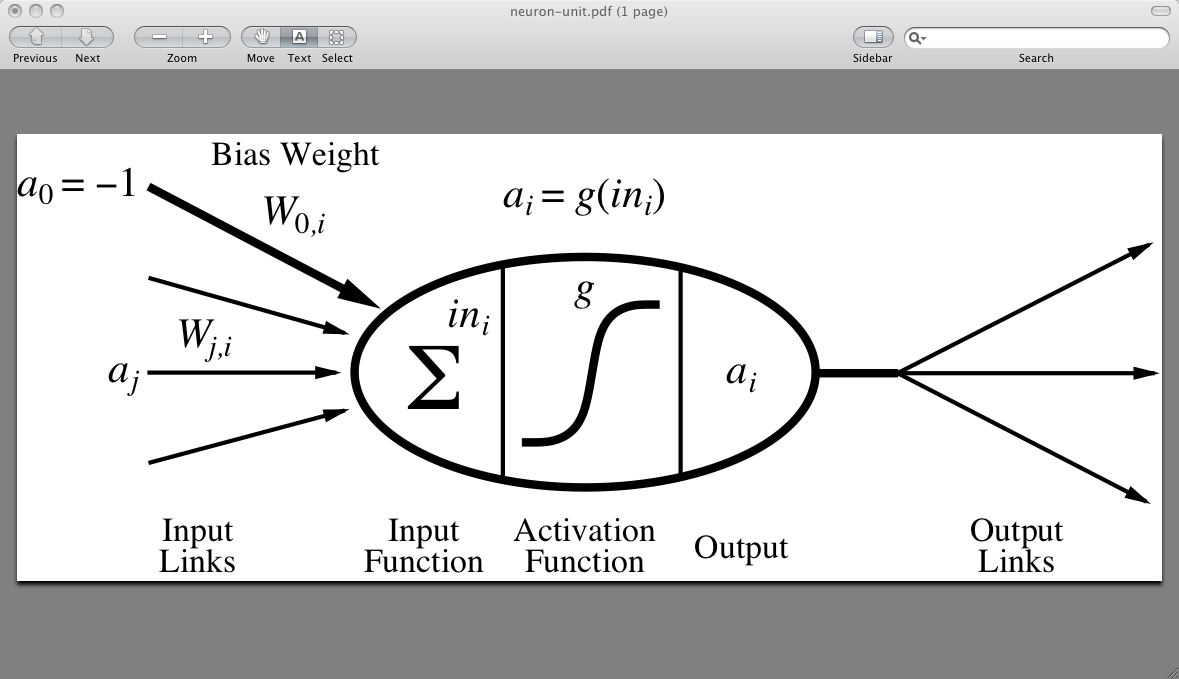
\includegraphics[width=3.5in]{./images/neuron-unit.png}
		\end{answer}
\question Figure \ref{fig:mystery-perceptron} is a schematic of a 3 input perceptron. Input $a_0$ is fixed at $a_0 = -1$, inputs $a_1$ and $a_2$ are binary. The perceptron uses a threshold activation function that outputs a 1 if the weighted sum of inputs is greater than 0 and a 0 otherwise. Define the \textbf{truth-table of the function} that this perceptron implements \emph{and} identify the \textbf{name of the function}. 
		\marks{8}
		\begin{answer}
		   {\Large
   \begin{tabular}{@{} ccc | c | c @{}}
      \multicolumn{3}{c}{Inputs} & $in_i$ & $a_i$ \\ \hline
      $a_0$ & $a_1$ & $a_2$ & $\sum_{j=0}^{2} w{j}{i} a_j$ & $\left( in_i  > 0\right)?(1):(0)$\\ \hline
      -1 & 1 & 1 & 0.5 & 1\\
      -1 & 1 & 0 & -0.5 & 0\\
      -1 & 0 & 1 & -0.5 & 0\\
      -1 & 0 & 0 & -1.5 & 0\\ \hline        
   \end{tabular}
   }\\
This perceptron implements the AND function.
		\end{answer}
	\end{enumerate}

\begin{figure}[h]
	\begin{center}
 		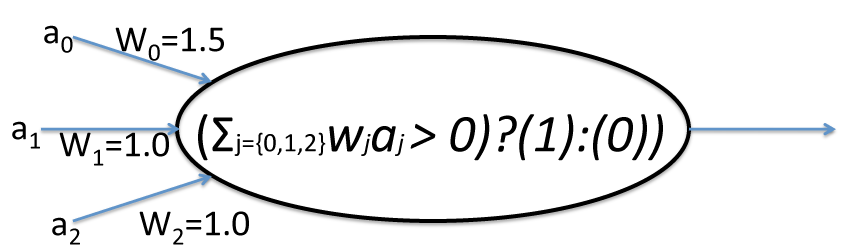
\includegraphics[width=4in]{./images/mystery-perceptron.png}
	\end{center}
		\caption{A 3 input perceptron. Input $a_0 = -1$, inputs $a_1$ and $a_2$ are binary. The perceptron uses a threshold activation function that outputs a 1 if the weighted sum of inputs is greater than 0 and a 0 otherwise.}
		\label{fig:mystery-perceptron}
\end{figure}


\end{document}
